\documentclass{beamer}
\usepackage[utf8]{inputenc}

\usepackage{utopia}
\setbeamerfont{caption}{series=\normalfont,size=\fontsize{8}{10}}

\usetheme{Madrid}
\usecolortheme{default}

\definecolor{RedCIMAT}{rgb}{0.44921875, 0.13671875, 0.234375}
\usecolortheme[named=RedCIMAT]{structure}

\setbeamertemplate{caption}[numbered]

\newcommand\Fontvi{\fontsize{10}{12.2}\selectfont}
\newcommand\FontEq{\fontsize{8}{12.2}\selectfont}

%------------------------------------------------------------
% Información de portada
\title[Detección de patologías pulmonares]{Detección de patologías pulmonares a través de modelos de aprendizaje profundo}
\subtitle{Tesis de Maestría}
\author[Oscar Esaú Peralta]{Oscar Esaú Peralta Rosales\\Director: Mariano JJ Rivera Meraz}
\institute[CIMAT]{Centro de Investigación en Matemáticas A.C.}
\date{Junio 2025}
\logo{\includegraphics[height=0.7cm]{logo.jpg}}
%------------------------------------------------------------

\AtBeginSection[]
{
  \begin{frame}
    \frametitle{Tabla de Contenido}
    \tableofcontents[currentsection]
  \end{frame}
}

\begin{document}

\frame{\titlepage}

\begin{frame}
\frametitle{Tabla de Contenido}
\tableofcontents
\end{frame}

% --- INTRODUCCIÓN ---

% 01-Introduccion_Presentacion_Tesis.tex
% Diapositivas de la sección Introducción

\section{Introducción}

\begin{frame}
\frametitle{Contexto: COVID-19 y Salud Pública}
\begin{itemize}
    \item La pandemia de COVID-19 ha tenido un impacto sin precedentes en la salud y el bienestar global.
    \item Saturación hospitalaria y vulnerabilidad de los trabajadores de la salud.
    \item Necesidad de métodos que apoyen el diagnóstico y tratamiento de enfermedades pulmonares.
\end{itemize}
\end{frame}

\begin{frame}
\frametitle{Historia y Desafíos del COVID-19}
\begin{itemize}
    \item COVID-19 surge en 2019 en Wuhan, China, y es declarada pandemia en marzo de 2020.
    \item La ciencia y tecnología son herramientas clave para enfrentar estos retos.
    \item Urgencia de métodos que agilicen el diagnóstico y tratamiento de enfermedades pulmonares.
\end{itemize}
\end{frame}

\begin{frame}
\frametitle{Diagnóstico por Imágenes y Aprendizaje Automático}
\begin{itemize}
    \item El análisis de imágenes de rayos X y TC es fundamental para el diagnóstico de enfermedades pulmonares.
    \item Modelos de inteligencia artificial ayudan a identificar patologías y visualizar regiones de interés.
    \item Mejoran la precisión y rapidez del diagnóstico, optimizando recursos hospitalarios.
\end{itemize}
\end{frame}

\begin{frame}
\frametitle{Limitaciones de los Métodos Actuales}
\begin{itemize}
    \item Sesgos por bases de datos pequeñas o no normalizadas.
    \item Enfoque limitado a enfermedades específicas.
    \item Falta de regulación, validación y explicabilidad de los modelos.
    \item Escasez de recursos para el procesamiento y etiquetado de imágenes.
\end{itemize}
\end{frame}

\begin{frame}
\frametitle{Desafíos y Necesidades}
\begin{itemize}
    \item Se requieren soluciones innovadoras que aprovechen el aprendizaje automático.
    \item Superar barreras técnicas, éticas y sociales para su aplicación clínica.
    \item Trabajo continuo para mejorar y diversificar las bases de datos de imágenes.
\end{itemize}
\end{frame}

\begin{frame}
\frametitle{Propuesta de la Tesis}
\begin{itemize}
    \item Desarrollo de modelos basados en redes neuronales convolucionales y Transformers.
    \item Detección de 15 patologías pulmonares, incluyendo COVID-19, usando imágenes de rayos X de diferentes fuentes.
    \item Evaluación mediante métricas de clasificación y visualización de regiones de interés.
\end{itemize}
\end{frame}


% --- MOTIVACIÓN Y OBJETIVOS ---

% 02-Motivacion_Objetivos_Presentacion_Tesis.tex
% Diapositivas de la sección Motivación y Objetivos

\section{Motivación y Objetivos}

\begin{frame}
\frametitle{Motivación: Problema Relevante}
\begin{itemize}
    \item La detección de COVID-19 y otras patologías pulmonares mediante imágenes de rayos X es un reto relevante y desafiante.
    \item El diagnóstico temprano y preciso mejora el pronóstico y tratamiento de los pacientes.
    \item Reduce el riesgo de contagio y la carga sobre el sistema de salud.
\end{itemize}
\end{frame}

\begin{frame}
\frametitle{Oportunidades y Retos Específicos}
\begin{itemize}
    \item Disponibilidad de grandes volúmenes de datos y avances en arquitecturas de deep learning.
    \item Integración de datos heterogéneos y adaptación a escenarios clínicos reales.
    \item Necesidad de modelos interpretables y validados clínicamente.
    \item Desafío de implementar soluciones en entornos con recursos limitados.
\end{itemize}
\end{frame}

\begin{frame}
\frametitle{Propuesta de la Tesis}
\begin{itemize}
    \item Desarrollo de modelos de Deep Learning capaces de detectar múltiples patologías pulmonares, incluyendo COVID-19.
    \item Uso de imágenes de rayos X provenientes de diferentes fuentes y regiones.
    \item Comparación de modelos basados en Transformers y CNNs, ambos con técnicas de Transfer Learning.
    \item Evaluación mediante métricas de clasificación y visualización de regiones de interés.
\end{itemize}
\end{frame}

\begin{frame}
\frametitle{Ventajas del Modelo Propuesto}
\begin{itemize}
    \item \textbf{Diagnóstico múltiple y holístico}: detección simultánea de varias patologías.
    \item \textbf{Robustez ante variabilidad de datos}: diferentes calidades, resoluciones y contrastes.
    \item \textbf{Interpretabilidad}: generación de mapas de calor para validar las predicciones.
    \item \textbf{Herramienta de apoyo}: para el análisis exploratorio, no reemplazo del médico.
\end{itemize}
\end{frame}

\begin{frame}
\frametitle{Objetivos Específicos}
\begin{itemize}
    \item Desarrollar modelos de clasificación multiclase para 15 patologías pulmonares.
    \item Implementar y comparar arquitecturas basadas en Transformers y CNNs.
    \item Evaluar la robustez de los modelos ante diferentes fuentes de datos.
    \item Generar visualizaciones interpretables para validación clínica.
\end{itemize}
\end{frame}


% --- MARCO TEÓRICO ---

% 04-Marco_Teorico_Presentacion_Tesis.tex
% Diapositivas de la sección Marco Teórico

\section{Marco Teórico}

\begin{frame}
\frametitle{Redes Neuronales Convolucionales (CNN)}
\begin{itemize}
    \item Las CNN son la base del análisis de imágenes médicas.
    \item Permiten extraer características espaciales relevantes de las imágenes.
    \item Se utilizan ampliamente en tareas de clasificación, segmentación y detección.
\end{itemize}
\begin{figure}[ht!]
    \centering
    \includegraphics[width=0.5\textwidth]{images/convolutional_network.png}
    \caption{Esquema de referencia de una red neuronal convolucional.}
\end{figure}
\end{frame}

\begin{frame}
\frametitle{Estructura de una red convolucional}
\begin{itemize}
    \item \textbf{Capa de Convolución}: Extrae características locales (bordes, texturas, patrones) mediante filtros (kernels).
    \item \textbf{Capa de Activación} (ReLU, LeakyReLU, etc.): Introduce no linealidad y elimina valores negativos.
    \item \textbf{Capa de Pooling}: Reduce la dimensionalidad conservando la información más relevante.
    \item \textbf{Capas Fully Connected} (Dense): Al final de la red, se aplanan los feature maps y se conectan a neuronas tradicionales para clasificación/regresión.
\end{itemize}
\end{frame}

\begin{frame}
\frametitle{Aplicaciones de una red convolucional}
\begin{itemize}
    \item \textbf{Clasificación de imágenes}: ResNet, VGG
    \item \textbf{Detección de objetos}: YOLO, Faster R-CNN
    \item \textbf{Segmentación semántica}: U-Net
    \item \textbf{Procesamiento de lenguaje natural}: CNNs para texto
\end{itemize}
\begin{figure}[ht!]
    \centering
    \includegraphics[width=0.4\textwidth]{images/cnn_applications.png}
    \caption{Aplicaciones de una red neuronal convolucional.}
\end{figure}
\end{frame}

\begin{frame}
\frametitle{ResNet50: Arquitectura Residual}
\begin{itemize}
    \item ResNet50 es una arquitectura profunda con 50 capas y conexiones residuales.
    \item Facilita el entrenamiento de redes muy profundas evitando el problema del desvanecimiento del gradiente.
    \item En esta tesis, ResNet50 se emplea como backbone para la extracción de características en imágenes de rayos X.
\end{itemize}
\begin{figure}[ht!]
    \centering
    \includegraphics[width=0.8\textwidth]{images/resnet50_architecture.png}
    \caption{Arquitectura base de un modelo ResNet.}
\end{figure}
\end{frame}

\begin{frame}
\frametitle{¿Por qué ResNet50 para esta tesis?}
\begin{itemize}
    \item \textbf{Buen rendimiento}: Probado en tareas de clasificación de imágenes médicas
    \item \textbf{Arquitectura establecida}: Ampliamente validada en la comunidad científica
    \item \textbf{Balance óptimo}: Entre profundidad y eficiencia computacional
    \item \textbf{Transfer learning efectivo}: Desde ImageNet a imágenes médicas
    \item \textbf{Capacidad de captura}: Características complejas en imágenes de rayos X
\end{itemize}
\end{frame}

\begin{frame}
\frametitle{Redes Neuronales Recurrentes (RNN)}
\begin{itemize}
    \item Las RNN procesan secuencias de datos, manteniendo información temporal.
    \item Son útiles para tareas donde el contexto previo es importante.
    \item Existen variantes como LSTM y GRU que mejoran la capacidad de memoria.
\end{itemize}
\begin{figure}[ht!]
    \centering
    \includegraphics[width=0.4\textwidth]{images/rnn.png}
    \caption{Grafo computacional de una RNN desenrollada.}
\end{figure}
\end{frame}

\begin{frame}
\frametitle{Mecanismos de Atención y Transformers}
\begin{itemize}
    \item Los Transformers revolucionaron el procesamiento de secuencias al permitir el procesamiento paralelo y el uso de atención múltiple (Multi-Head Attention).
    \item Los mecanismos de atención permiten al modelo enfocarse en partes relevantes de la entrada.
    \item Vision Transformer (ViT) aplica estos conceptos a imágenes.
\end{itemize}
\begin{figure}[ht!]
    \centering
    \includegraphics[width=0.42\textwidth]{images/attention.png}
    \caption{Ilustración del mecanismo de atención obtenida de la publicación "All you need is Attention".}
\end{figure}
\end{frame}

\begin{frame}
\frametitle{Mecanismos de Atención y Transformers}
\begin{figure}[ht!]
    \centering
    \includegraphics[width=0.8\textwidth]{images/vit.png}
    \caption{Ilustración del modelo ViT obtenida de la publicación "An Image is worth 16X16 words".}
\end{figure}
\end{frame}

\begin{frame}
\frametitle{Mecanismos de Atención y Transformers}
\begin{table}[h!]
    \centering
    \fontsize{7}{8}\selectfont
    \begin{tabular}{|p{2.5cm}|p{3cm}|p{3cm}|}
        \hline
        \textbf{Característica} & \textbf{Transformers (con atención)} & \textbf{RNNs / BiRNNs} \\
        \hline
        Paralelización & Totalmente paralelizable durante el entrenamiento & Procesamiento secuencial, difícil de paralelizar \\
        \hline
        Dependencias a largo plazo & Captura relaciones entre tokens distantes fácilmente & Difícil de mantener contexto a largo plazo \\
        \hline
        Velocidad de entrenamiento & Más rápido gracias a la paralelización & Más lento por la naturaleza secuencial \\
        \hline
        Escalabilidad & Escala bien con grandes cantidades de datos y capas & Escalabilidad limitada por problemas de gradiente \\
        \hline
        Multi-head attention & Permite aprender múltiples representaciones en paralelo & No tiene un mecanismo equivalente \\
        \hline
        Representación contextual rica & Cada token se representa en función de todos los demás & Representación más local y secuencial \\
        \hline
    \end{tabular}
    \caption{Comparación entre Transformers y RNNs/BiRNNs en tareas de modelado de secuencias}
    \label{tab:comparacion_transformers_rnns}
\end{table}
\end{frame}

\begin{frame}
\frametitle{Resumen del Marco Teórico}
\begin{itemize}
    \item Se presentan dos modelos de arquitecturas para el procesamiento y detección de patologías pulmonares
        \begin{itemize}
            \item Convolucionales (ResNet50). Extrayendo características de las imágenes, a través de la convolución de filtros.
            \item Modelos basados en atención (ViT). Procesando imágenes como secuencias de datos, manteniendo información temporal.
        \end{itemize}
\end{itemize}
\end{frame}

% \begin{frame}
% \frametitle{Resumen del Marco Teórico}
% \begin{table}[h!]
%     \centering
%     \fontsize{8}{9}\selectfont
%     \begin{tabular}{|p{2.5cm}|p{3cm}|p{3cm}|}
%         \hline
%         \textbf{Aspecto} & \textbf{CNNs} & \textbf{Vision Transformers (ViT)} \\
%         \hline
%         Extracción de características & Local y jerárquica & Global desde el inicio \\
%         \hline
%         Interpretación espacial & Implícita por la estructura convolucional & Necesita codificación posicional \\
%         \hline
%         Campo receptivo (Receptive field) & Aumenta con la profundidad & Global desde la primera capa \\
%         \hline
%         Transferencia de conocimiento & Muy efectiva con preentrenamiento & Requiere mucho preentrenamiento para funcionar bien \\
%         \hline
%     \end{tabular}
%     \caption{Comparación entre redes convolucionales (CNNs) y Vision Transformers (ViT)}
%     \label{tab:comparacion_cnns_vit}
% \end{table}
% \end{frame}


% --- METODOLOGÍA ---

% 05-Metodologia_Presentacion_Tesis.tex
% Diapositivas de la sección Metodología

\section{Metodología}

\begin{frame}
\frametitle{Flujo General de la Metodología}
\begin{itemize}
    \item Desarrollo de modelos de aprendizaje profundo para la detección de 15 patologías pulmonares en rayos X.
    \item Dos enfoques principales: ResNet50 (CNN) y Vision Transformer (ViT).
    \item Proceso estructurado: preprocesamiento, entrenamiento, evaluación y extensión a nuevas patologías.
\end{itemize}
\end{frame}

\begin{frame}
\frametitle{Bases de Datos y Composición}
\begin{itemize}
    \item Uso del dataset ChestX-ray14 (112,120 imágenes, 30,805 pacientes, 14 patologías).
    \item Extensión con imágenes de COVID-19 y saludables.
    \item Re-etiquetado de datos usando modelos automáticos para mejorar la calidad de las etiquetas.
\end{itemize}
\end{frame}

\begin{frame}
\frametitle{Preprocesamiento de Imágenes}
\begin{itemize}
    \item Redimensionamiento a $1024 \times 1024$ y $384 \times 384$ píxeles según el modelo.
    \item Normalización y estandarización de intensidades.
    \item Data augmentation: rotaciones, traslaciones, escalados y flips para robustez.
\end{itemize}
\end{frame}

\begin{frame}
\frametitle{Entrenamiento: Transfer Learning y Fine-Tuning}
\begin{itemize}
    \item ResNet50 y ViT preentrenados en ImageNet.
    \item Tres etapas: (1) Transfer learning (cambio de la capa de salida), (2) Fine-tuning de las últimas capas, (3) Full-tuning de toda la red.
    \item Permite adaptar modelos generales a tareas médicas específicas con menos datos.
\end{itemize}
\end{frame}

\begin{frame}
\frametitle{Arquitectura de los Modelos}
\begin{columns}
\column{0.5\textwidth}
\textbf{ResNet50}
\begin{itemize}
    \item Red convolucional profunda con conexiones residuales.
    \item Extrae características espaciales de las radiografías.
\end{itemize}
\column{0.5\textwidth}
\textbf{Vision Transformer (ViT)}
\begin{itemize}
    \item Divide la imagen en parches y los procesa como una secuencia.
    \item Utiliza mecanismos de atención para capturar relaciones globales.
\end{itemize}
\end{columns}
\begin{figure}[ht!]
    \centering
    \includegraphics[width=0.5\textwidth]{../Chapters/2. Transformer/Figures/transformer/encoder.jpg}
    \caption{Esquema de codificador Transformer (ViT).}
\end{figure}
\end{frame}

\begin{frame}
\frametitle{Evaluación y Métricas}
\begin{itemize}
    \item División de datos en entrenamiento, validación y prueba.
    \item Métricas: AUC, precisión, recall, F1-score y matriz de confusión.
    \item Visualización de resultados: mapas de calor y curvas ROC.
\end{itemize}
\begin{figure}[ht!]
    \centering
    \includegraphics[width=0.3\textwidth]{../Chapters/2. Transformer/Figures/transformer/fastformer.png}
    \caption{Ejemplo de visualización de atención en modelos tipo Transformer.}
\end{figure}
\end{frame}

\begin{frame}
\frametitle{Extensión y Generalización}
\begin{itemize}
    \item El modelo puede ser extendido fácilmente a nuevas patologías (ejemplo: tuberculosis).
    \item El proceso de re-etiquetado y entrenamiento permite adaptar el sistema a diferentes escenarios clínicos.
    \item Resultados competitivos frente al estado del arte en todas las patologías evaluadas.
\end{itemize}
\end{frame}


% --- RESULTADOS ---

% 05-Resultados_Presentacion_Tesis.tex
% Diapositivas de la sección Resultados

\section{Resultados}

\begin{frame}
\frametitle{Resumen de Resultados}
\begin{itemize}
    \item \textbf{Modelo ResNet50}: AUC-ROC Global-15 = 0.852
    \begin{itemize}
        \item Supera a CheXNet (0.841) y otros métodos del estado del arte
        \item COVID-19: AUC-ROC = 0.991, F1-Score = 0.799
    \end{itemize}
    \item \textbf{Modelo ViT}: AUC-ROC Global-15 = 0.791
    \begin{itemize}
        \item COVID-19: AUC-ROC = 0.982, F1-Score = 0.801
        \item Limitado por resolución de imagen (384x384)
    \end{itemize}
    \item \textbf{Comparación con radiólogos}: Los modelos superan a radiólogos en 6/15 patologías
\end{itemize}
\end{frame}

\begin{frame}
\frametitle{Comparación con el Estado del Arte}
\begin{table}[ht!]
    \centering
    \tiny
    \begin{tabular}{|l||c|c|c|c|c|c|c|l|}
        \hline
        \multicolumn{1}{|c||}{Patología}	&	\multicolumn{5}{c|}{\bf Modelos comparativos}    &\multicolumn{2}{c|}{\bf Propuestas} & 	\\
        \cline{2-9}
                        &	CRAL	&	DR-CNN	&	TSNC	& LgMeta & CheXNet	& CNN	    & ViT & 	Radiol.	\\
        \hline\hline
        Cardiomegaly	&	0.880	&	0.801	&	0.887	&	0.875	&\bf{0.923}	&	0.875	& 0.866 &	0.888	\\
        Emphysema	    &	0.908	&	0.773	&	0.930	&	0.895	&	0.937	&\bf{0.938}	& 0.866 &   0.911	\\
        Effusion	    &	0.829	&	0.797	&	0.831	&	0.822	&\bf{0.864}	&	0.850	& 0.791 &   0.900*	\\
        Hernia	        &	0.917	&	0.748	&	0.921	&\bf{0.937}	&	0.916	&	0.855	& 0.843 &   0.985*	\\
        Infiltration	&	0.702	&\bf{0.751}	&	0.703	&	0.694	&	0.734	&	0.740	& 0.621 &	0.734	\\
        Mass	        &	0.834	&	0.760	&	0.833	&	0.820	&\bf{0.868}	&	0.831	& 0.768 &	0.886*	\\
        Nodule	        &	0.773	&	0.741	&	0.798	&	0.747	&	0.780	&\bf{0.806}	& 0.704 &	0.899*	\\
        Atelectasis	    &	0.781	&	0.766	&	0.785	&	0.763	&\bf{0.809}	&	0.794	& 0.734 &	0.808	\\
        Pneumothorax	&	0.729	&	0.778	&	0.731	&	0.840	&	0.889	&\bf{0.906}	& 0.842 &	0.940*	\\
        Pleural-Thick.	&	0.778	&	0.759	&	0.782	&	0.763	&	0.806	&\bf{0.820}	& 0.765 &	0.779	\\
        Pneumonia	    &	0.857	&	0.800	&\bf{0.881}	&	0.731	&	0.768	&	0.863	& 0.738 &	0.823	\\
        Fibrosis	    &	0.830	&	0.765	&	0.833	&	0.816	&	0.805	&\bf{0.852}	& 0.810 &	0.897*	\\
        Edema	        &	0.850	&	0.820	&	0.849	&	0.846	&\bf{0.888}	&	0.879	& 0.828 &	0.910*	\\
        Consolidation	&	0.754	&	0.787	&	0.754	&	0.749	&\bf{0.790}	&	0.776	& 0.715 &	0.841*	\\
        \hline
        COVID-19	    &	---	    &	---	    &	---	    &	---	    &	---	    &\bf{0.991}	& 0.982 &	---	    \\
        Healthy	        &	---	    &	---	    &	---	    &	0.727	&	---	    &\bf{0.736}	& 0.705 &	---	    \\
        \hline\hline
        Global-14	    &	0.816	&	0.775	&	0.823	&	0.807	&	0.841	&\bf{0.842}	& 0.778 &	0.872*	\\
        Global-15	    &	---	    &	---	    &	---	    &	---	    &	---	    &\bf{0.852}	& 0.791 &	---	    \\
        \hline
    \end{tabular}
    \caption{Valores correspondientes a la métrica AUC-ROC para las 15 patologías y muestras saludables.}
    \label{table_roc_auc}
\end{table}
\end{frame}

\begin{frame}
\frametitle{Resultados por Patología - ResNet50 vs ViT}
\begin{table}[ht!]
    \centering
    \tiny
    \begin{tabular}{|l||c|c|c|c||c|c|c|c|}
        \hline
        {\bf Patología} & \multicolumn{4}{c||}{\bf ResNet50} & \multicolumn{4}{c|}{\bf ViT} \\
        \cline{2-9}
         & AUC-PR & AUC-ROC & F1-Score & Acc. & AUC-PR & AUC-ROC & F1-Score & Acc. \\
        \hline\hline
        Cardiomegaly    & 0.290 & 0.875 & 0.324 & 0.911 & 0.253 & 0.866 & 0.324 & 0.928 \\
        Emphysema       & 0.413 & 0.938 & 0.350 & 0.886 & 0.246 & 0.866 & 0.319 & 0.924 \\
        Effusion        & 0.494 & 0.850 & 0.527 & 0.807 & 0.401 & 0.791 & 0.434 & 0.807 \\
        Hernia          & 0.050 & 0.855 & 0.051 & 0.957 & 0.036 & 0.843 & 0.064 & 0.971 \\
        Infiltration    & 0.382 & 0.740 & 0.458 & 0.711 & 0.256 & 0.621 & 0.235 & 0.724 \\
        Mass            & 0.290 & 0.831 & 0.340 & 0.877 & 0.227 & 0.768 & 0.296 & 0.900 \\
        Nodule          & 0.249 & 0.806 & 0.299 & 0.876 & 0.157 & 0.704 & 0.209 & 0.908 \\
        Atelectasis     & 0.336 & 0.794 & 0.387 & 0.815 & 0.271 & 0.734 & 0.325 & 0.840 \\
        Pneumothorax    & 0.447 & 0.906 & 0.496 & 0.852 & 0.359 & 0.842 & 0.430 & 0.880 \\
        Pleural-Thick   & 0.157 & 0.820 & 0.217 & 0.852 & 0.125 & 0.765 & 0.197 & 0.881 \\
        Pneumonia       & 0.425 & 0.863 & 0.274 & 0.856 & 0.104 & 0.738 & 0.144 & 0.732 \\
        Fibrosis        & 0.106 & 0.852 & 0.154 & 0.910 & 0.070 & 0.810 & 0.134 & 0.932 \\
        Edema           & 0.187 & 0.879 & 0.193 & 0.788 & 0.120 & 0.828 & 0.180 & 0.877 \\
        Consolidation   & 0.150 & 0.776 & 0.234 & 0.754 & 0.118 & 0.715 & 0.171 & 0.836 \\
        \hline
        COVID-19        & 0.844 & 0.991 & 0.799 & 0.969 & 0.859 & 0.982 & 0.801 & 0.973 \\
        Healthy         & 0.691 & 0.736 & 0.496 & 0.712 & 0.634 & 0.705 & 0.537 & 0.703 \\
        \hline\hline
        Global-14       & 0.284 & 0.842 & 0.307 & 0.847 & 0.196 & 0.778 & 0.247 & 0.867 \\
        Global-15       & 0.321 & 0.852 & 0.340 & 0.855 & 0.240 & 0.791 & 0.284 & 0.874 \\
        \hline
    \end{tabular}
    \caption{Resumen del rendimiento de los modelos propuestos basados en \textit{ResNet50} y \textit{ViT} para cada patología.}
    \label{table:res-vit-model-covid}
\end{table}
\end{frame}

\begin{frame}
\frametitle{Curvas ROC - ResNet50}
\begin{figure}[ht!]
    \centering
    \includegraphics[width=0.5\textwidth]{../Chapters/4. ViT-Lung/images/ROC_AUC.pdf}
    \caption{Curvas ROC del modelo ResNet50 para todas las patologías.}
\end{figure}
\end{frame}

\begin{frame}
\frametitle{Curvas ROC - ViT}
\begin{figure}[ht!]
    \centering
    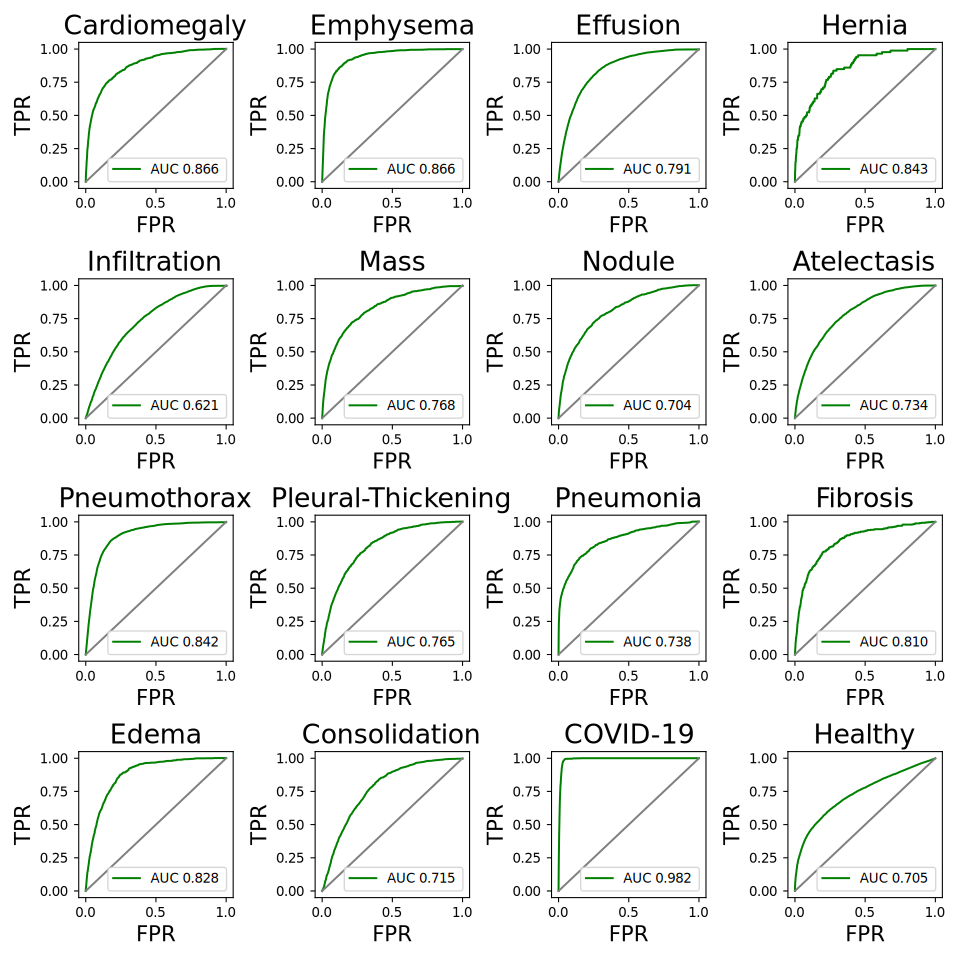
\includegraphics[width=0.5\textwidth]{../Chapters/4. ViT-Lung/images/ROC_AUC_ViT.pdf}
    \caption{Curvas ROC del modelo ViT. Mantiene buen rendimiento a pesar de menor resolución.}
\end{figure}
\end{frame}

\begin{frame}
\frametitle{Visualización de Atención - GradCAM}
\begin{figure}[ht!]
    \centering
    \includegraphics[width=0.8\textwidth]{../Chapters/4. ViT-Lung/images/vlgrid.png}
    \caption{Ejemplos de visualización GradCAM: Cardiomegaly, Pneumonia, Mass y COVID-19. Las regiones rojas indican las áreas de mayor atención del modelo.}
\end{figure}
\end{frame}

\begin{frame}
\frametitle{Comparación con Radiólogos Humanos}
\begin{table}[ht!]
    \centering
    \tiny
    \begin{tabular}{|l||l|c|l|}
        \hline
                        &	Method	&	AUC-ROC	& Radiol.	\\
        \hline\hline
        Cardiomegaly	&	CheXNet	    & 0.923 &   0.888	\\
        Emphysema	    &	Proposal    & 0.938	&   0.911	\\
        Effusion	    &	CheXNet	    & 0.864 &   0.900*	\\
        Hernia	        &	LargeMeta   & 0.937	&   0.985*	\\
        Infiltration	&	DR-CNN	    & 0.751 &	0.734	\\
        Mass	        &	CheXNet	    & 0.868	&	0.886*	\\
        Nodule	        &	Proposal    & 0.806	&	0.899*	\\
        Atelectasis	    &	CheXNet	    & 0.809 &	0.808	\\
        Pneumothorax	&	Proposal    & 0.906 &	0.940*	\\
        Pleural-Thick.	&	Proposal    & 0.820	&	0.779	\\
        Pneumonia	    &	TSNC	    & 0.881 &	0.823	\\
        Fibrosis	    &	Proposal    & 0.852 &	0.897*	\\
        Edema	        &	CheXNet	    & 0.888 &	0.910*	\\
        Consolidation	&	CheXNet	    & 0.790 &	0.841*	\\
        COVID-19	    &	Proposal    & 0.991 &	------	\\
        \hline
    \end{tabular}
    %}
    \caption{Comparativo por patología de los modelos de deep learning con mejor rendimiento contra
             el rendimiento de los radiólogos humanos. Los radiólogos lideran en 8 de las 15
             patologías.}
    \label{table_dl_human}
\end{table}
\end{frame}

\begin{frame}
\frametitle{Extensión a Tuberculosis - Resultados}
\begin{itemize}
    \item \textbf{Clasificador binario para tuberculosis}
    \begin{itemize}
        \item F1-Score: 0.707
        \item Accuracy: 0.846
        \item Verdaderos positivos: 388/488 casos
    \end{itemize}
    \item \textbf{Análisis en modelo de 15 patologías}
    \begin{itemize}
        \item ResNet50: 480 casos detectados como COVID-19, 93 como neumonía
        \item ViT: 481 casos como COVID-19, 2 como neumonía
        \item Comportamiento esperado debido a similitudes radiológicas
    \end{itemize}
\end{itemize}
\end{frame}

\begin{frame}
\frametitle{Análisis de Limitaciones y Fortalezas}
\begin{columns}
\column{0.5\textwidth}
\textbf{ResNet50 - Fortalezas:}
\begin{itemize}
    \item Mayor resolución (1024x1024)
    \item Mejor rendimiento global
    \item Más épocas de entrenamiento
    \item Arquitectura probada
\end{itemize}

\column{0.5\textwidth}
\textbf{ViT - Fortalezas:}
\begin{itemize}
    \item Convergencia más rápida
    \item Menos épocas necesarias
    \item Atención global
    \item Arquitectura moderna
\end{itemize}

\textbf{Limitación principal:}
\begin{itemize}
    \item Consumo de memoria alto
    \item Resolución limitada (384x384)
\end{itemize}
\end{columns}
\end{frame}

% \begin{frame}
% \frametitle{Conclusiones de Resultados}
% \begin{itemize}
%     \item \textbf{Rendimiento excepcional}
%     \begin{itemize}
%         \item ResNet50 establece nuevo estándar (AUC-ROC Global-15: 0.852)
%         \item COVID-19: AUC-ROC de 0.991 (ResNet50) y 0.982 (ViT)
%     \end{itemize}
%     \item \textbf{Superación del estado del arte}
%     \begin{itemize}
%         \item Lidera en 5 patologías específicas
%         \item Supera a radiólogos en 6/15 patologías
%     \end{itemize}
%     \item \textbf{Versatilidad demostrada}
%     \begin{itemize}
%         \item Extensión exitosa a tuberculosis
%         \item Interpretabilidad clínica con GradCAM
%     \end{itemize}
%     \item \textbf{Impacto clínico potencial}
%     \begin{itemize}
%         \item Herramienta valiosa para apoyo diagnóstico
%         \item Capacidad de adaptación a nuevas patologías
%     \end{itemize}
% \end{itemize}
% \end{frame}


% --- CONCLUSIONES Y TRABAJO FUTURO ---

% 06-Conclusiones_TrabajoFuturo_Presentacion_Tesis.tex
% Diapositivas de la sección Conclusiones y Trabajo Futuro

\section{Conclusiones y Trabajo Futuro}

% \begin{frame}
% \frametitle{Conclusiones de Resultados}
% \begin{itemize}
%     \item \textbf{Rendimiento excepcional}
%     \begin{itemize}
%         \item ResNet50 establece nuevo estándar (AUC-ROC Global-15: 0.852)
%         \item COVID-19: AUC-ROC de 0.991 (ResNet50) y 0.982 (ViT)
%     \end{itemize}
%     \item \textbf{Superación del estado del arte}
%     \begin{itemize}
%         \item Lidera en 5 patologías específicas
%         \item Supera a radiólogos en 6/15 patologías
%     \end{itemize}
%     \item \textbf{Versatilidad demostrada}
%     \begin{itemize}
%         \item Extensión exitosa a tuberculosis
%         \item Interpretabilidad clínica con GradCAM
%     \end{itemize}
%     \item \textbf{Impacto clínico potencial}
%     \begin{itemize}
%         \item Herramienta valiosa para apoyo diagnóstico
%         \item Capacidad de adaptación a nuevas patologías
%     \end{itemize}
% \end{itemize}
% \end{frame}

% \begin{frame}
% \frametitle{Logros Principales}
% \begin{itemize}
%     \item \textbf{Desarrollo exitoso} de dos modelos de aprendizaje profundo para 15 patologías pulmonares
%     \begin{itemize}
%         \item ResNet50: AUC-ROC Global-15 = 0.852 (nuevo estándar incluyendo COVID-19)
%         \item ViT: AUC-ROC Global-15 = 0.791 (alto rendimiento en COVID-19)
%     \end{itemize}
%     \item \textbf{Desempeño destacado en COVID-19}
%     \begin{itemize}
%         \item ResNet50: AUC-ROC = 0.991, F1-Score = 0.799
%         \item ViT: AUC-ROC = 0.982, F1-Score = 0.801
%     \end{itemize}
%     \item \textbf{Superación del estado del arte} en múltiples patologías
%     \item \textbf{Capacidad de extensión} demostrada con tuberculosis
% \end{itemize}
% \end{frame}

\begin{frame}
\frametitle{Contribuciones Científicas}
Muy buen rendimiento en 15 patologías pulmonares estableciendo un nuevo estándar con la inclusion de COVID-19.
\begin{itemize}
    \item \textbf{Superación del estado del arte}
    \begin{itemize}
        \item Lidera en 5 patologías específicas. Supera a radiólogos en 6/15 patologías.
    \end{itemize}
    \item \textbf{Introducción de Vision Transformers} en análisis de imágenes médicas.
    \begin{itemize}
        \item Demostración de viabilidad vs CNNs tradicionales como una posible alternativa.
    \end{itemize}
    \item \textbf{Estrategia de Transfer Learning} de tres etapas:
    \begin{itemize}
        \item Entrenamiento inicial (backbone congelado).
        \item Fine-tuning (últimas capas).
        \item Full-tuning (modelo completo).
    \end{itemize}
\end{itemize}
\end{frame}

\begin{frame}
\frametitle{Capacidad de Extensión Demostrada}
\begin{itemize}
    \item \textbf{Extensión a tuberculosis} exitosa
    \begin{itemize}
        \item Aprovechamiento de backbone pre-entrenado.
        \item Comparable con métodos específicos para tuberculosis.
    \end{itemize}
    \item \textbf{Proceso de extensión} simple y eficiente:
    \begin{itemize}
        \item Reutilización del backbone pre-entrenado.
        \item Adición de rama clasificadora específica.
        \item Entrenamiento solo de nuevas capas.
    \end{itemize}
    \item \textbf{Plataforma versátil} para inclusión de futuras patologías.
\end{itemize}
\end{frame}


\begin{frame}
\frametitle{Limitaciones Identificadas}
\begin{itemize}
    \item \textbf{Calidad y representatividad de datos}
    \begin{itemize}
        \item Diversidad de datos limitada.
        \item Posibles sesgos en etiquetado y distribución de patologías.
    \end{itemize}
    \item \textbf{Falta de validación clínica}
    \begin{itemize}
        \item No probado en entornos hospitalarios reales
        \item Necesidad de certificación médica
    \end{itemize}
    \item \textbf{Recursos computacionales caso ViT}
    \begin{itemize}
        \item Limitado a 384x384 píxeles
        \item Consumo de memoria alto
        \item Tiempo de entrenamiento extenso y necesidad de más datos.
    \end{itemize}
\end{itemize}
\end{frame}

\begin{frame}
\frametitle{Líneas de Trabajo Futuro}
\begin{itemize}
    \item \textbf{Exploración de nuevas arquitecturas}
    \begin{itemize}
        \item EfficientNet y DenseNet avanzados
        \item Variantes mejoradas de Vision Transformers
        \item Arquitecturas híbridas CNN-Transformer
        \item Arquitecturas de atención más sofisticadas
    \end{itemize}
    \item \textbf{Datos y Validación}
    \begin{itemize}
        \item Mejora de bases de datos; inclusion de más patologías, datos de alta calidad y anotación precisa.
        \item Validación clínica rigurosa.
        \item Regulación y certificación para uso clínico.
    \end{itemize}
\end{itemize}
\end{frame}

\begin{frame}
\frametitle{Líneas de Trabajo Futuro - Multimodalidad}
\begin{itemize}
    \item \textbf{Integración de múltiples modalidades}
    \begin{itemize}
        \item Tomografía computarizada (CT)
        \item Resonancia magnética (MRI)
        \item Ultrasonido pulmonar
    \end{itemize}
    % \item \textbf{Modelos multimodales}
    % \begin{itemize}
    %     \item Fusión de información de diferentes fuentes
    %     \item Arquitecturas que procesen múltiples tipos de imagen
    %     % \item Técnicas de alineación multimodal
    % \end{itemize}
    \item \textbf{Datos clínicos adicionales}
    \begin{itemize}
        \item Historiales médicos
        \item Síntomas del paciente
        \item Resultados de laboratorio
    \end{itemize}
\end{itemize}
\end{frame}

\begin{frame}
\frametitle{Líneas de Trabajo Futuro - Herramientas Visuales}
\begin{itemize}
    % \item \textbf{Mejora de técnicas de interpretabilidad}
    % \begin{itemize}
    %     \item GradCAM avanzado
    %     \item SHAP (SHapley Additive exPlanations)
    %     \item LIME (Local Interpretable Model-agnostic Explanations)
    % \end{itemize}
    \item \textbf{Interfaces de usuario clínicas}
    \begin{itemize}
        \item Dashboards para radiólogos
        \item Sistemas de reporte automatizado
        \item Integración con PACS (Picture Archiving and Communication System)
    \end{itemize}
    \item \textbf{Visualizaciones interactivas}
    \begin{itemize}
        \item Exploración de regiones de interés
        \item Comparación de múltiples modelos
    \end{itemize}
\end{itemize}
\end{frame}

% \begin{frame}
% \frametitle{Impacto Clínico y Social}
% \begin{itemize}
%     \item \textbf{Acceso a diagnóstico especializado}
%     \begin{itemize}
%         \item Regiones con recursos limitados
%         \item Reducción de tiempos de espera
%         \item Mejora de eficiencia del sistema de salud
%     \end{itemize}
%     \item \textbf{Herramientas de triaje}
%     \begin{itemize}
%         \item Clasificación automática de urgencias
%         \item Priorización de casos críticos
%         \item Apoyo en emergencias médicas
%     \end{itemize}
%     \item \textbf{Adaptabilidad epidemiológica}
%     \begin{itemize}
%         \item Extensión a nuevas patologías emergentes
%         \item Adaptación a contextos locales
%         \item Respuesta rápida a crisis sanitarias
%     \end{itemize}
% \end{itemize}
% \end{frame}

\begin{frame}
\frametitle{Conclusiones Finales}
\begin{itemize}
    \item \textbf{Nuevos estándares establecidos}
    \begin{itemize}
        \item Rendimiento superior al estado del arte
        \item Viabilidad de Vision Transformers en medicina
        \item Capacidad de extensión demostrada
    \end{itemize}
    \item \textbf{Contribución al campo}
    \begin{itemize}
        \item Metodología reproducible con base de datos diversa
        \item Plataforma para futuras investigaciones
    \end{itemize}
    \item \textbf{Impacto potencial}
    \begin{itemize}
        \item Herramientas valiosas para diagnóstico
    \end{itemize}
    \item \textbf{Próximos pasos}
    \begin{itemize}
        \item Validación clínica rigurosa
        \item Desarrollo de herramientas visuales
        \item Integración en práctica médica como herramienta de apoyo
    \end{itemize}
\end{itemize}
\end{frame}


% --- AGRADECIMIENTOS ---

% \input{07-Agradecimientos_Presentacion_Tesis}

\begin{frame}
\begin{center}
    Gracias por su atención.
\end{center}
\end{frame}

\end{document}
